\documentclass[11.5pt,twoside]{report}
\usepackage[T1]{fontenc} %times new roman
\usepackage{mathptmx}
\usepackage{polski}
%\usepackage{biblatex}
\usepackage[utf8]{inputenc} %polskie znaki
\linespread{1.1}
\usepackage[inner=3.18cm,outer=2.54cm,]{geometry} %marginesy
\usepackage{graphicx} 
\usepackage{titlesec}
\renewcommand*{\figurename}{Fig.} %zmienia etykietowanie z "Rys." na "Fig."
\usepackage{chngcntr}
\counterwithout{figure}{chapter} %ustawia jedno numerowanie figur w całym dokumencie
\setlength{\belowcaptionskip}{-5pt} %zmienia odległość między podpisem figury a tekstem
\usepackage[font=small,labelfont=bf]{caption} %formatowanie podpisów figur: mała czcionka, "Fig." boldem
\setlength{\parindent}{1.5em}
\setlength{\parskip}{0em}

\usepackage{lipsum} %usuwa "Rozdział" z nazwy rozdziału
\makeatletter
\def\@makechapterhead#1{
	\vspace*{0\p@}
	{\parindent \z@ \raggedright \normalfont
		\ifnum \c@secnumdepth >\m@ne
		\if@mainmatter
		\LARGE\bfseries \thechapter.\space%
		\fi
		\fi
		\interlinepenalty\@M
		\LARGE \bfseries #1\par\nobreak
		\vskip 15\p@     %odległość między tytułem a tekstem
}}
\makeatother

\usepackage{multicol} %kolumny

\newenvironment{localsize}[1] %tworzenie środowiska localsize (lokalna zmiana wielkości czcionki)
{%
	\clearpage
	\let\orignewcommand\newcommand
	\let\newcommand\renewcommand
	\makeatletter
	\input{bk#1.clo}%
	\makeatother
	\let\newcommand\orignewcommand
}
{%
	\clearpage
}

%\usepackage[autostyle]{csquotes}
%\addbibresource{biblatex-examples.bib}

%
%
%
%
\begin{document}
	
	\tableofcontents
	
	\chapter{Kenozoiczna historia termiczna centralnej Europy}
	
W czasie mezozoiku i kenozoiku górna skorupa Europy zachowała układ scalonych bloków, utworzony podczas orogenez: kaledońskiej i waryscyjskiej. Dolna skorupa i płaszcz litosferyczny uległy zaś znacznemu przeobrażeniu i, w konsekwencji, odmłodzeniu. Od pó\'{z}nej kredy (ok. 80 mln lat temu), granica litosfery i astenosfery pod Europą centralną migrowała ku powierzchni ziemi (Fig. 1). 

\begin{figure}[h]
	\centering
	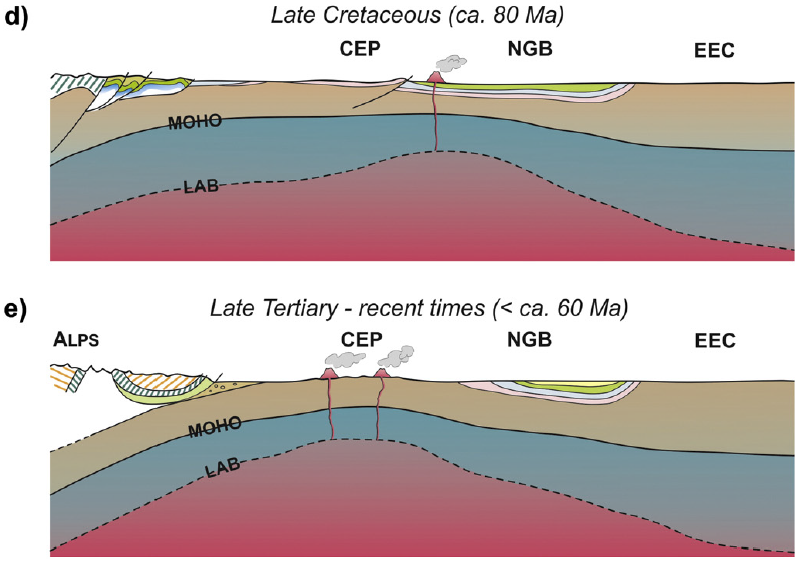
\includegraphics[width=0.5\linewidth]{../Termika/Meier2016}
	\caption{Schemat ewolucji płaszcza litosferycznego pod Europą. \textit{Na górze} późna kreda (ok. 80 mln lat temu), \textit{na dole} późny trzeciorzęd (ok. 60 mln lat temu) do dziś. \textit{CEP} platforma środkowoeuropejska, \textit{NGB} basen północnoniemiecki, \textit{EEC} kraton wschodnioeuropejski (Meier et al., 2016).}
	\label{Fig.}
\end{figure}
	
	\section{Zlodowacenia plejstoceńskie}
	
	\section{Orogeneza alpejska}
	
	\subsection{Wypiętrzenie Karpat}
	
	\subsection{Powstanie systemu ryftów na kontynencie europejskim}
	
Wykształcenie się w kenozoiku systemu ryftów na kontynencie europejskim (ang. ECRIS -- \textit{European Cenozoic Rift System}, Fig. 1) było prawdopodobnie spowodowane reakcją hercyńskiego podłoża na akrecję bloków kontynetalnych podczas orogenezy alpejskiej (Ulrych et al., 2002). W paleocenie siły kompresyjne odpowiedzialne za fałdowanie łańcuchów Alp i Pirenejów oddziaływały na litosferę w strefie do 1700 km na północ od głównych frontów deformacji. U początków eocenu naprężenia kompresyjne na przedgórzu Alp zmniejszały się względem naprężeń powodujacych fałdowanie Pirenejów, wskutek czego doszło do otwarcia systemu ryftów w międzypłytowym reżimie kompresyjnym. Główna faza riftingu przypadła na oligocen, kiedy to proces ten był kontrolowany przez działające w kierunku północnym naprężenia powstające w strefach kolizyjnych Alp i Pirenejów. Od wczesnego miocenu, po ustaniu subdukcji w Pirenejach i otwarciu basenu algiersko-prowansalskiego w zachodniej części Morza Śródziemnego, rozwój ECRIS był podtrzymywany przez naprężenia oddziaływujące w kierunku północnym i północno-zachodnim związane z powstawaniem eksternidów alpejskich (D\`{e}zes et al., 2004). Uniesienie astenosfery (w rodzaju pióropusza płaszcza) pod ścienioną litosferą alpejskiego przedpola umożliwiło rozpoczęcie wytapiania zmetasomatyzowanego płaszcza (Ulrych et al., 2002).

\begin{figure}[h]
	\centering
	\includegraphics[width=0.7\linewidth]{../Termika/dezes2004}
	\caption{Rozmieszczenie rowów tektonicznych (\textit{jasnoszary}) powstałych w kenozoiku na przedpolu Alp i Pirenejów oraz związanych z nimi pól wulkanicznych (\textit{czarny}), linia przerywana -- front deformacji alpejskich; \textit{BF} Schwarzwald, \textit{BG} rów Bresse, \textit{EG} rów Eger, \textit{FP} Wyżyna Frankońska, \textit{HG} rowy heskie, \textit{LG} rów Limagne, \textit{LRG} rów Dolnego Renu, \textit{URG} rów Górnego Renu, \textit{OW} Odenwald, \textit{VG} Wogezy (D\`{e}zes et al., 2004).}
\label{Fig.}
\end{figure}

Aktywność tektoniczna związana z ryftowaniem oraz wulkanizm w rowach należących do ECRIS wygasały w różnym czasie. Rowy Masywu Centralnego i Rodanu stały się nieaktywne z początkiem miocenu, podczas gdy system rowów reńskich wykazuje aktywność do dzisiaj (D\`{e}zes et al., 2004). Ryft Egeru powstał w fazie ekstensji, która dotknęła Masyw Czeski na przełomie eocenu i miocenu. Rozmieszczenie intruzji magmowych świadczy o postępującym ku wschodowi rozwoju ryftu. Ostatni etap rozwoju ryftu przypadł na 24-16(?) mln lat temu i był to czas kształtowania się współcześnie obserwowanej struktury rowu ograniczonego przez uskoki (Adamovič i Coubal, 1999) -- od południa przez strefę uskokową Czeskiego Średniogórza, a od północy przez strefę uskokową Rudaw (Cajz i Valečka, 2010).

%sprawdzić te nazwy stref uskokowych po polsku
	
	\subsection{Wulkanizm}
	
Zjawiska wulkaniczne są zarówno bezpośrednią przyczyną podwyższenia lokalnej charakterystyki termicznej, jak i przejawem regionalnych fenomenów natury litosferycznej czy płaszczowej (odpowiedzialnych za wulkanizm), wpływających na wartości parametrów termicznych na danym obszarze. Bepośredni wpływ wulkanizmu na temperaturę litosfery wyraża się w powstawaniu aureoli termicznych wokół ciał magmowych intrudujących w skały górotworu. Dokładna ilościowa ocena wpływu termicznego intruzji na otaczający górotwór musi uwzględniać wiele czynników, m. in. geometrię ciała magmowego, różnice w przewodności cieplnej ośrodków, konwekcję w magmie, możliwość zainstnienia konwekcji wód porowych w skałach otoczenia; w mniejszym stopniu reakcje metamorficzne (dehydratacja, rozkład węglanów i inne) czy wolatylizację wód porowych (Annen, 2017). Grubość aureoli wokół intruzji odzwierciedla dynamikę tworzenia intruzji -- w wyniku pojedynczego zdarzenia bąd\'{z} na drodze wieloetapowego procesu (Galushkin, 1997). Wpływ termiczny intruzji na skały otoczenia może być ewaluowany w badaniach refleksyjności witrynitu (jako miernika przetworzenia termicznego materii organicznej; np. Annen, 2017; Fjeldskaar et al., 2008). 

	\subsubsection{Wulkanizm karpacki i panoński}

Na obszarze poddanym przekształceniom podczas orogenzey alpejskiej pojawiły się w kenozoiku związane genetycznie z procesami górotwórczymi zjawiska wulkaniczne. Alpejskie wydarzenia orogeniczne kredy i paleogenu, kiedy miało miejsce skracanie litosfery oceanicznej Oceanu Tetydy na drodze subdukcji, nie skutkowały w tym czasie zjawiskami wulkanicznymi. Przyczyną tego był panujący wówczas w domenie karpacko-panońskiej reżim kompresyjny oraz znaczna grubość litosfery, niepoddanej jeszcze wówczas ekstensji. Jednakże, zaistniała wówczas metasomatyzacja płaszcza, możliwa dzięki dehydratacji subdukowanych fragmentów litosfery. Uwodnienie płaszcza pozwoliło na zmniejszenie temperatury generacji stopu, który zaczął migrować ku powierzchni wraz z rozpoczęciem etapu ekstensji we wczesnym miocenie, około 20 mln lat temu. Stopy płaszczowe, docierając do skorupy, powodowały jej topnienie i tworzenie magm krustalnych. W etapie ekstensji generacja magm płaszczowych podtrzymywana była przez mechanizm wytapiania dekompresyjnego, a dalsza subdukcja wpływała na skład magm (Haragi i Lenkey, 2007).

%zob. Konecny et al., 2002   

Wulkanizm kenozoiczny (neogeński) domeny karpacko-panońskiej był fenomenem wieloetapowym. Kolejne jego fazy cechowały się różnym chemizmem oraz miejscem występowania. Ogółem, zjawiska te datowane są na okres 21-0,1 mln lat temu, przy czym centrum aktywności wulkanicznej przesuwało się w czasie z zachodu na wschód (Lexa et al., 2010; P\'{e}cskay et al., 1995). Zmienny charakter chemiczny zjawisk wulkanicznych odzwierciedlał różne epizody tektoniczne w rejonie. Wyróżnia się trzy główne etapy wulkanizmu karpacko-panońskiego w neogenie: 1) miocen (około 20-11 mln lat temu): kwaśny wulkanizm kalcialkaliczny -- ignimbryty i tufy basenu panońskiego i transylwańskiego; 2) środkowy miocen - czwartorzęd (17-0,2 mln lat temu): pośredni (między felsytowym a maficznym) wulkanizm kalcialkaliczny (niezwiązany genetycznie z wulkanizmem felsytowym miocenu), z końcową fazą bazaltową -- andezyty (w tym andezyty pienińskie) występujące w łuku wulkanicznym po wewnętrznej stronie Karpat fliszowych, rozciągającym się od basenu dunajskiego po rumuński kompleks Călimani-Gurghiu-Harghita; 3) wulkanizm alkaliczny (dwie fazy: 17-7 i 6-0,5 mln lat temu) -- sporadyczne wystąpienia na całym obszarze karpacko-panońskim -- od szoszonitów kapratu (17-16 mln lat temu) do bazaltów alkalicznych i szoszonitów czwartorzędowych (P\'{e}cskay et al., 1995).
  
Geneza zjawisk wulkanicznych w regionie Karpat i basenu panońskiego w oczywisty sposób wydaje się być powiązana z historią tektoniczną tego obszaru. Kwestią dyskusji jest, czy współcześnie obserwowane wysokie wartości parametrów termicznych związane są z postulowanym przez niektórych badaczy (jakich?) pióropuszem płaszcza w podłożu panońskim. Sygnatury izotopowe HIMU i FOZO, którymi charakteryzują się alkaliczne skały magmowe basenu panońskiego i Karpat oraz charakterystyka termiczna regionu przemawiają za hipotezą istnienia pióropusza. Jednakże, taki skład izotopowy może być efektem metasomatozy (niekoniecznie zaś pióropusza płaszcza), a wysokie wartości strumienia cieplnego wyjaśnia również ścienienie skorupy podczas ekstensji i płytkie usytuowanie LAB (ang. \textit{litosphere-astenophere boundary}). Wpływ epizodu ekstensyjnego na wartości strumienia cieplnego wygasa po ok. 100 milionach lat (McKenzie, 1978 --> znalezc), więc w płaszczu pod basenem panońskim wciąż mogą istnieć warunki do generacji stopu (prawdopodobnie w wyniku podwyższenia temperatury przez inną niż piórpusz płaszcza nieokreśloną perturbację natury płaszczowej). Przeciwko hipotezie pióropusza płaszcza pod basenem panońskim przemawia także brak kopułowatego wyniesienia regionu w topografii, sporadyczny charakter i rozproszenie przestrzenne przejawów wulkanizmu panońskiego oraz niskie tempo produkcji magmy (Harangi i Lenkey, 2007).    
  
Wpływ intruzji na zwiększenie temperatur i strumienia cieplnego w ich pobliżu wygasa w ciągu kilku milionów lat (Fowler and Nisbet, 1982; Horv\'{a}th et al., 1986, za: Lenkey, 2002 --> zmienic). Anomalnie wysokie wartości strumienia cieplnego na obszarze Karpat Wschodnich mogą być wiązane z zakończoną około 0,1 miliona lat temu aktywnością wulkaniczną na tym obszarze. Śródkowomioceński wulkanizm kalcialkaliczny i zjawiska wulkaniczne występujące w przeszłości wzdłuż łuku Karpat po jego wewnętrznej stronie nie powinny mieć więc współcześnie wpływu na podwyższenie parametrów termicznych. Emisja ciepła radiogenicznego z powstałych wówczas utworów wulkanicznych, z uwagi na względnie małą zawartość pierwiastków promieniotówrczych, nie ma istotnego wpływu ilościowego na strumień cieplny. Obserwowane wysokie wartości temperatur i strumienia cieplnego mają więc zapewne \'{z}ródło w dolnej skorupie bąd\'{z} płaszczu; domniemywać można, że to samo \'{z}ródło odpowiadało za panoński wulkanizm mioceński. Kwaśny wulkanizm plioceński i plejstoceński, ze względu na epizodyczny charakter aktywności i niewielką objętość związanych z nim ciał magmowych, nie miał istotnego wpływu na lokalną termikę litosfery (Lenkey et al., 2002).

Na obszarze Polski kenozoiczna aktywność wulkaniczna domeny karpacko-panońskiej zaznaczyła się w Pieninach, gdzie występują mioceńskie (11-13 mln lat temu) andezyty (np. Góra Wżar). Skały te, współcześnie odpreparowane przez erozję, pierwotnie powstały jako intruzje, płytko usytuowane pod powierzchnią terenu. Możliwe, że w miocenie istniały na obszarze Pienin aktywne wulkany, ale nie jest to czytelnie poświadczone w zapisie kopalnym (Krzemińska i Awdankiewicz, 2011).

	\subsubsection{Wulkanizm sudecki i ryftu Egeru}

Kenozoiczne zjawiska wulkaniczne Sudetów odpowiedzialne były za powstanie na obszarze Polski dolnośląskiej formacji bazaltowej. Genetycznie wulkanizm sudecki jest zbliżony (spośród formacji środkowoeuropejskich) do pól wulkanicznych w Niemczech i Czechach związanych z rowem Egeru (Oh\v{r}y), a także, w mniejszym stopniu, ze strefą uskokową Łaby i Odry (Puziewicz et al., 2011). Do formacji tych należą: wulkanity niecki żytawskiej na terenie Niemiec (B\"{u}chner et al., 2015), na obszarze Czech: Czeskie Średniogórze, Doupovské hory, południowo-zachodni kraniec rowu Egeru na pograniczu Czech i Górnego Palatynatu (Fig. 1). Formacje te zaliczane są do środkowoeuropejskiej prowincji wulkanicznej -- rozciągajacej się na przedpolu Alpidów (od pasma Eifel po Śląsk) strefy występowania śródpłytowych pól wulkanicznych. Według Kopeck\'{y}'ego (zrodlo?), rozwój zjawisk wulkanicznych na tym obszarze jest związany z rozległą strefą ryftową, rozciągającą się od Renu, przez Niemcy i Czechy, po zachodnią Polskę (\textit{ECRIS} -- \textit{European Cenozoic Rift System}). Aktywność wulkaniczna w obrębie środkowoeuropejskiej prowincji wulkanicznej rozpoczęła się pod koniec kredy, z początkiem riftingu (melilitytowy kompleks Osečná na przecięciu głównego uskoku łużyckiego i rowu Egeru, 68-59 mln lat temu; Ulrych et al., 2008; Ulrych et al., 2000) i trwała do czwartorzędu (Eifel, Masyw Centralny i zachodni kraniec rowu Egeru). Według Meier et al. (2016), ryfty tworzące ECRIS miały od poczatku charakter pasywny i wystepowanie wulkanizmu na ich obszarze jest raczej zjawiskiem wtórnym, związanym ze ścienieniem litosfery. Przeto, należy domniemywać, że wulkanizm ECRIS i kenozoiczne uniesienie LAB w środkowej Europie jest skutkiem procesów płaszczowych (Meier et al., 2016).

\begin{figure}[h]
	\centering
	\includegraphics[width=0.7\linewidth]{../Termika/lvf}
	\caption{Pola wulkaniczne kenozoicznej środkowoeuropejskiej prowincji wulkanicznej. \textit{CS} Czeskie Średniogórze, \textit{DH} Doupovsk\'{e} hory, \textit{HDS} heidelberski rój dajek, \textit{LVF} łużyckie pole wulkaniczne, \textit{WOR} zachodni rów Oh\v{r}y. Masywy waryscyjskie: \textit{A} Ardeny, \textit{BF} Szwarcwald, \textit{H} Harz, \textit{O} Odenwald, \textit{RM} Masyw Reński, \textit{S} Spessart, \textit{V} Wogezy (B\"{u}chner et al., 2015).} 
	\label{Fig.}
\end{figure}

W opinii wielu badaczy (jakich?), pola wulkaniczne środkowoeuropejskiej prowincji wulkanicznej reprezentują śródpłytowy typ wulkanizmu. Według Lebedev et al. (2006), ten typ wulkanizmu występuje w miejscach, gdzie głębokość do astenosfery jest mniejsza niż na pobliskim obszarze kratonicznym. Zgodnie z tą hipotezą, w takich warunkach w astenosferze wytwarza się subhoryzontalny przepływ, a w miejscu, gdzie litosfera jest ścieniona, dochodzi do dekompresyjnego wytapiania i, w konsekwencji, do pojawienia się wulkanizmu. Charakterystyczne dla wulkanizmu typu śródpłytowego są: monogenetyczność stopów, ich niewielka objętość i krótki okres aktywności wulkanów. Stopy (na ogół bazaltowe; alkaliczne bąd\'{z} pośrednie) są zazwyczaj generowane w płaszczu (w stosunkowo krótkim czasie), przy czym w czasie migracji przez skorupę może następować mixing bąd\'{z} dyferencjacja. Erupcja wulkanów śródpłytowych następuje na skutek wzrostu ciśnienia w ciele magmowym ponad wartość ciśnienia litostatycznego (Kereszturi i Németh, 2013). Występowanie pól wulkanicznych w obrębie ECRIS koreluje z obszarem kenozoicznego ścienienia litosfery. Dzięki ekstensji możliwa była wysokotemperaturowa, efektywna pod względem stopnia wytopienia skał generacja stopów o wysokiej zawartości krzemionki (Meier et al., 2016).

Kenozoiczny wulkanizm na Dolnym Śląsku związany był z wschodnim krańcem ryftu Egeru (Krzemińska i Awdankiewicz, 2011). W obrębie dolnośląskiej formacji bazaltowej wulkanity występują w kilku głównych centrach: 1) blok przedsudecki; 2) przy krawędzi Sudetów Środkowych; 3) w zachodniej części Sudetów (związane z północną częścią ryftu Egeru), a ponadto na terenie depresji kredy opolskiej oraz jako pojedyncze wystąpienia w Karkonoszach i Górach Złotych. Aktywność wulkaniczna miała miejsce przede wszystkim w oligocenie i miocenie (31-4 mln lat temu; Badura i Przybylski, 2004).

Ogółem, na Dolnym Śląsku znajduje się około 300 stanowisk występowania wulkanitów kenozoicznych -- są to głównie niewielkie żyły i kominy, fragmenty potoków lawowych i piroklastyki. Sporadycznie występują dobrze zachowane stożki wulkaniczne, np. w Graczach k. Opola i w Targowicy k. Strzelina (Krzemińska i Awdankiewicz, 2011). Obserwowane w badaniach grawimetrycznych i magnetycznych anomalie bazaltowe mogą świadczyć o znacznym zasięgu utworów wulkanicznych występujących płytko przy powierzchni skorupy ziemskiej (Badura i Przybylski, 2004). Pod względem litologicznym, w obrębie kenozoicznych wulkanitów Sudetów polskich najpowszechniej występują bazanity, nefelinity i bazalty alkaliczne. Badania geochemiczne tych skał wskazują, że stopy, z których powstały, miały pochodzenie astenosferyczne lub/i litosferyczne i były produktem wytapiania perydotytów granatonośnych i spinelowych bąd\'{z} wytworzyły się w efekcie topnienia w strefie przejściowej między tymi facjami (Puziewicz et al., 2011).

%Lanberger et al 2006  

%stratygrafia wulkanitów dś na podst Birkenmajera
  
%Wierzchołowski, 1993 --> geneza magm (BN) 
%puziewicz 2011 - o płaszczu litosferycznym
%http://www.geolodzy.uni.wroc.pl/bazalty/index.html

	
	\subsection{Powstanie zapadlisk przed- i śródgórskich}
	
Wypiętrzeniu Karpat towarzyszyło powstanie rejonów zapadliskowych, do których zalicza się zapadlisko przedkarpackie i basen panoński. Ograniczony łańcuchami Alp, Karpat i Gór Dynarskich basen panoński (Fig. 1) dzieli się na wiele podjednostek, z których największą i centralną jest obniżenie Wielkiej Niziny Węgierskiej. Oprócz Wielkiej Niziny Węgierskiej, do panońskiego systemu basenów należą również mniejsze baseny, m. in. basen dunajski (Mała Nizina Węgierska), basen Grazu (styryjski), których granice wyznaczają masywy gór wyspowych. Baseny znajdujące się na obrzeżach domeny panońskiej (basen wiedeński, transylwański, transkarpacki) położone są w bezpośrednim sąsiedztwie granicy płaszczowin eoalpejskich (występujących w podłożu basenu panońskiego) oraz nasunięć fliszu karpackiego (Kováč et al., 2007; Fodor et al., 1999).

\begin{figure}[h]
	\centering
	\includegraphics[scale=0.7]{"../Termika/kovac et al"}
	\caption{Jednostki georegionalne w otoczeniu basenu panońskiego (Kováč et al., 2007).}
	\label{Fig.}
\end{figure}

\subsubsection{Basen panoński}

Panoński system basenowy powstał w wyniku serii zdarzeń tektonicznych, mających miejsce od środkowego triasu do dziś. W mezozoiku obszar współczesnego basenu panońskiego wypełniał ocean Neotetydy, w którego podłożu rozwijały się strefy ryftowe. Pod koniec jury doszło do zderzenia terranów Alcapa i Tisza-Dacja, których kontakt współcześnie wyznacza śródwowęgierska strefa uskokowa. Utworzone wówczas płaszczowiny stanowią podłoże współczesnego basenu panońskiego. W miocenie rozpoczęła się faza ekstensji basenu w jego wewnętrznych partiach, jednocześnie z aktywnością subdukcyjną w strefach brzeżnych (Csontos i V\"{o}r\"{o}s, 2004). Po etapie intensywnej ekstensji dalszy rozwój basenu następował na drodze subsydencji termicznej, będącej efektem kontrakcji termicznej litosfery podczas jej stygnięcia. Taki dwuetapowy model rozwoju basenu ekstensyjnego (faza intensywnej ekstensji, a po niej bardziej pasywna faza subsydencji) potwierdzają badania sejsmiki refleksyjnej i luster tektonicznych w uskokach na obszarze basenu panońskiego. Obecnie (od pó\'{z}nego pliocenu) teren basenu panońskiego znajduje się w reżimie kompresyjnym, w którym jego brzeżne partie na wschodzie i zachodzie ulegają wynoszeniu (Horv\'{a}th i Cloething, 1996). 

Litosferę basenu panońskiego cechują wyjątkowo wysokie wartości strumienia cieplnego, przekraczające 80 ${mW/m}^{2}$ (Boldizsar, 1964). Mierzone wartości strumienia cieplnego mieszczą się w przedziale 50-130 ${mW/m}^{2}$, a średnia wynosi okolo 100 ${mW/m}^{2}$ (Horv\'{a}th et al., 2015). Takie warunki termiczne są pozostałością po mioceńskim etapie ekstensji, w trakcie którego doszło do silnego wygrzania litosfery (Lenkey et al., 2017). Ze zjawiskami termicznymi związany był neogeńsko-czwartorzędowy (21-0,1 mln lat temu) wulkanizm o charakterze kwaśnym i kalcialkalicznym. W czasie geologicznym wulkanizm ten migrował z zachodu na wschód (Lexa et al., 2010). 

Największe wartości strumienia cieplnego rejestrowane są w miejscach wyniesień podłoża między głębszymi basenami Wielkiej Niziny Węgierskiej (B\'{e}k\'{e}si et al., 2017). 

\begin{figure}[h]
	\centering
	\includegraphics[width=0.7\linewidth]{"../Termika/grubosc skorupy"}
	\caption{Rozkład grubości skorupy w regionie panońskim (Horváth et al., 2015).}
	\label{fig:grubosc-skorupy}
\end{figure}

 W związku ze znaczną subsydencją, basen panoński był miejscem intensywnej sedymentacji, w wyniku której doszło do nagromadzenia miąższych (0,1-7 km) osadów neogeńskich, o~charakterze morskim, deltowym, jeziornym i rzecznym (T\'{o}th i Alm\'{a}si, 2001). Intensywna sedymentacja jako proces oraz sposób występowania warstwy osadowej w profilu geologicznym mają istotny wpływ na kształtowanie strumienia cieplnego docierającego do powierzchni ziemi. Wysokie tempo sedymentacji zmniejsza wartości strumienia cieplnego rejestrowane przy powierzchni ziemi (Lenkey et al., 2017; Horv\'{a}th et al., 2015). Wartości strumienia cieplnego z poprawką na sedymentację są o 10-30 \% wyższe od bezpośrednio obserwowanych (Lenkey et al., 2002). Ponadto, skały osadowe są środowiskiem występowania zjawisk hydrogeologicznych, które mają pewien wpływ na strumień cieplny. Infiltracja wód meteorycznych (szczególnie w miejscach wychodni powierzchniowych wysoko porowatych wapieni) przyczynia się do znacznego spadku rejestrowanych wartości strumienia cieplnego, np. w Dynarydach zewnętrznych do 30 ${mW/m}^{2}$ (Horv\'{a}th et al., 2015). Ogrzane wody meteoryczne docierając z powrotem ku powierzchni ziemi odpowiadają za powstawanie gorących \'{z}ródeł, licznie występujących na obszarze panońskim. Pomiar energii termicznej niesionej przez gorące wody może posłużyć do oszacowania konwekcyjnego transportu ciepłą, a dodanie tej wartości do obserwowanego strumienia cieplnego daje w wyniku wartość strumienia cieplnego w warunkach niezaburzonych przez cyrkulację wód (Lenkey et al., 2017). Cyrkulacja wód podziemnych jest również przyczyną zaburzeń kondukcyjnego przepływu ciepła płaszczowego ku powierzchni ziemi. Grawitacyjny przepływ wód podziemnych oraz rozwijanie się komórek konwekcyjnych w obrębie tych wód mogą zmienić wartości powierzchniowego strumienia cieplnego (Horv\'{a}th et al., 2015). 
 
 W obrębie wypełnienia osadowego basenu panońskiego (neogeńskiego i mezozoicznego) wykształciły się dwa systemy wodonośne, przedzielone warstwą oligoceńskich osadów marglistych o niskiej przepuszczalności. W wyższym systemie dominujący czynnik powodujący przepływ jest natury grawitacyjnej, związany z topografią. Niższy system (cyrkulacja w skałach położonych głębiej) poddany jest oddziaływaniom tektonicznym o charakterze kompresyjnym, które są przyczyną wytworzenia nadciśnienia w wodach porowych (T\'{o}th i Alm\'{a}si, 2001). Innym wytłumaczeniem takiego stanu rzeczy jest duże tempo sedymentacji, niezrównoważone z tempem kompakcji i odprowadzania wód porowych, przez co ciśnienie w wodach porowych danego ośrodka narasta (Horv\'{a}th et al., 2015). Oba systemy nie są w pełni izolowane, jako że uskoki stanowią miejsca ułatwionego przepływu solanek z niższego systemu ku powierzchni (T\'{o}th i Alm\'{a}si, 2001). Mezozoiczne formacje węglanowe z wychodniami na powierzchni ziemi stanowią odrębny system hydrogeologiczny z przzepływem kontrolowanym grawitacyjnie (Horv\'{a}th et al., 2015). 
 
 Wysokie ciśnienia i temperatury panujące w obrębie skał niższego systemu wodonośnego, w połączeniu z dużą porowatością tych utworów, umożliwiają rozwój konwekcyjnego przepływu wód (Horv\'{a}th et al., 2015). 
 
 \subsubsection{Zapadlisko przedkarpackie}
 
 	\chapter{Modele termiczne dla obszaru Polski -- historia badań}
 
	\chapter{Rozpoznanie strumienia cieplnego na obszarze Polski}
 
% 	\chapter{Teoretyczne podstawy modelowania stanu termicznego litosfery}
 
% 	\chapter{Parametry materiałowe skał}
 
% 	\chapter{Rozpoznanie struktury litosfery na obszarze Polski}
 
% 	\chapter{Ocena perspektyw modelowania stanu termicznego litosfery na obszarze Polski}

%\nocite{*}
%\printbibliography
%\bibliographystyle{plain}
%0\bibliography{bibliografia}

\chapter*{Bibliografia}
\addcontentsline{toc}{chapter}{Bibliografia} 

%znalezc, co tu sie stalo

\begin{multicols}{3} %kolumny
	
\begin{localsize}{10}
	
\parindent=0pt
\parskip=\smallskipamount

Annen, C., 2017. Factors Affecting the Thickness of Thermal Aureoles. Front. Earth Sci. 5, 1614.

Békési, E. et al., 2017. Subsurface temperature model of the Hungarian part of the Pannonian Basin. Global and Planetary Change.

Boldizsár, T., 1964. Terrestrial heat flow in the Carpathians. J. Geophys. Res. 69 (24), 5269–5275.

Csontos, L., Vörös, A., 2004. Mesozoic plate tectonic reconstruction of the Carpathian region. Palaeogeography, Palaeoclimatology, Palaeoecology 210 (1), 1–56.

Fjeldskaar, W. et al., 2008. Thermal modelling of magmatic intrusions in the Gjallar Ridge, Norwegian Sea: implications for vitrinite reflectance and hydrocarbon maturation. Basin Research (20), 143–159. 

Fodor, L. et al., 1999. Tertiary tectonic evolution of the Pannonian Basin system and neighbouring orogens: A new synthesis of palaeostress data. Geological Society, London, Special Publications 156 (1), 295–334. 

Galushkin, Y., 1997. Thermal effects of igneous intrusions on maturity of organic matter: A possible mechanism of intrusion. Organic Geochemistry 26 (11-12), 645–658. 

Harangi, S., Lenkey, L., 2002. Genesis of the Neogene to Quaternary volcanism in the Carpathian-Pannonian region: Role of subduction, extension, and mantle plume. Geological Society of America (Special Paper 418), 67–92.

Horváth, F., Cloetingh, S., 1996. Stress-induced late-stage subsidence anomalies in the Pannonian basin. Tectonophysics 266 (1-4), 287–300. 

Horváth, F. et al., 2015. Evolution of the Pannonian basin and its geothermal resources. Geothermics 53, 328–352. 

Kováč, M. et al., 2007. Badenian evolution of the Central Paratethys Sea: paleogeography, climate and eustatic sea-level changes. Geologia Carpathica 58 (6), 579–606.

Lenkey, L. et al., 2002. Geothermics of the Pannonian basin and its bearing on the neotectonics. Stephan Mueller Special Publication Series (3), 29–40.

Lexa, J. et al., 2010. Neogene-Quaternary Volcanic forms in the Carpathian-Pannonian Region: A review. Open Geosciences 2 (3), 15.

Pécskay, Z. et al., 1995. Space and time distribution of Neogene-Quaternary volcanism in the Carpatho-Pannonian region. Acta Vulcanologica (7 (2)), 15–28.

Toth, J., Almasi, I., 2001. Interpretation of observed fluid potential patterns in a deep sedimentary basin under tectonic compression: Hungarian Great Plain, Pannonian Basin. Geofluids 1 (1), 11–36.

\end{localsize}

\end{multicols}

\end{document}
